This section presents the results of comparing the proposed no-communication algorithm with Tarry's algorithm, as well as analyzing Tarry's performance against its variants. We evaluate these approaches on different datasets, detailed in Section \ref{section_datasets}, to observe how distinct graph properties influence the efficiency of the solutions. Section \ref{section_result_no_comm} discusses the performance of the no-communication algorithms. Section \ref{section_result_tarry} then presents the analysis of Tarry's algorithm and its variants.

\section{Datasets for Algorithm Evaluation} 
\label{section_datasets}

This section describes the datasets used to evaluate the performance of the algorithms. The datasets consist of two types of graphs:

\begin{itemize} 
    \item Perfect Mazes: The dataset of perfect mazes \cite{Naeem2021} is the same as the one used by \citen{Arthur2023} and includes 250 mazes for each of four sizes: 10x10, 20x20, 30x30, and 40x40.
    \item Random Trees: The dataset of random trees was generated using the $random\_$ $unlabeled\_tree$ method from NetworkX \cite{Hagberg2008}. This dataset includes 250 trees for each of the following sizes: 100, 250, 500, 1000, and 1500 nodes. After generating the graphs, nodes that did not contribute any new decisions to the tree (specifically, nodes with only two edges) were contracted by adding an edge between their two neighbors and then removed. 
\end{itemize}

The analysis focuses on datasets and sizes that yield significant results, while all generated graphs can be found in the appendix.


\section{No-Communication Algorithms Performance}
\label{section_result_no_comm}

\subsection{Metrics for Analysis}
\label{subsection_no_comm_metrics}

This section focuses on the results for the no-communication algorithms, which include the proposed algorithm, its Backward Interval Filling variant, and Tarry's algorithm for comparison. Although Tarry's algorithm involves communication, it serves as a baseline to assess the efficiency of the no-communication strategies.


The metrics used in this comparison are:

\begin{itemize}
    \item Steps Taken by the Pioneer: This measures the number of steps needed by the first agent to find the goal, serving as a key indicator of exploration efficiency.
    \item Fraction Explored Before the Pioneer Found the Goal: This indicates the proportion of the graph covered by the agents before the goal was reached, providing insight into how well the agents dispersed during exploration.
\end{itemize}
    
These metrics together give a clear view of the algorithm's efficiency and how exploration patterns vary across different graph structures and sizes.

\subsection{Perfect Maze Results} 
\label{subsection_no_comm_maze_results}


The results for all maze sizes (10x10, 20x20, 30x30, and 40x40) are presented in Figures \ref{fig_no_comm_steps_all_sizes_maze} and \ref{fig_no_comm_fraction_all_sizes_maze}, showing how the different no-communication algorithms perform across various maze dimensions. Figure \ref{fig_no_comm_steps_all_sizes_maze} represents the steps taken by the pioneer, while Figure \ref{fig_no_comm_fraction_all_sizes_maze} shows the explored fraction before the goal was found, allowing for a detailed comparison of exploration efficiency and coverage.

\begin{figure}[H]
    \centering
    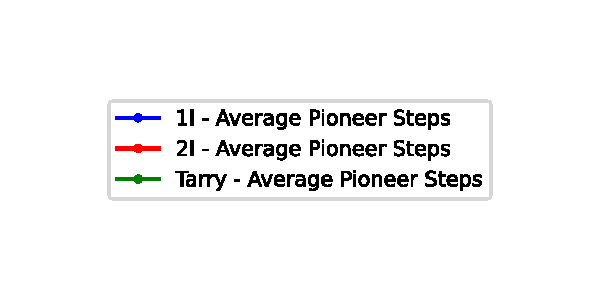
\includegraphics[width=0.8\textwidth]{Cap3/no_comm_steps_legend.pdf}
    \vspace{1em}
    \begin{minipage}[b]{0.45\textwidth}
        \centering
        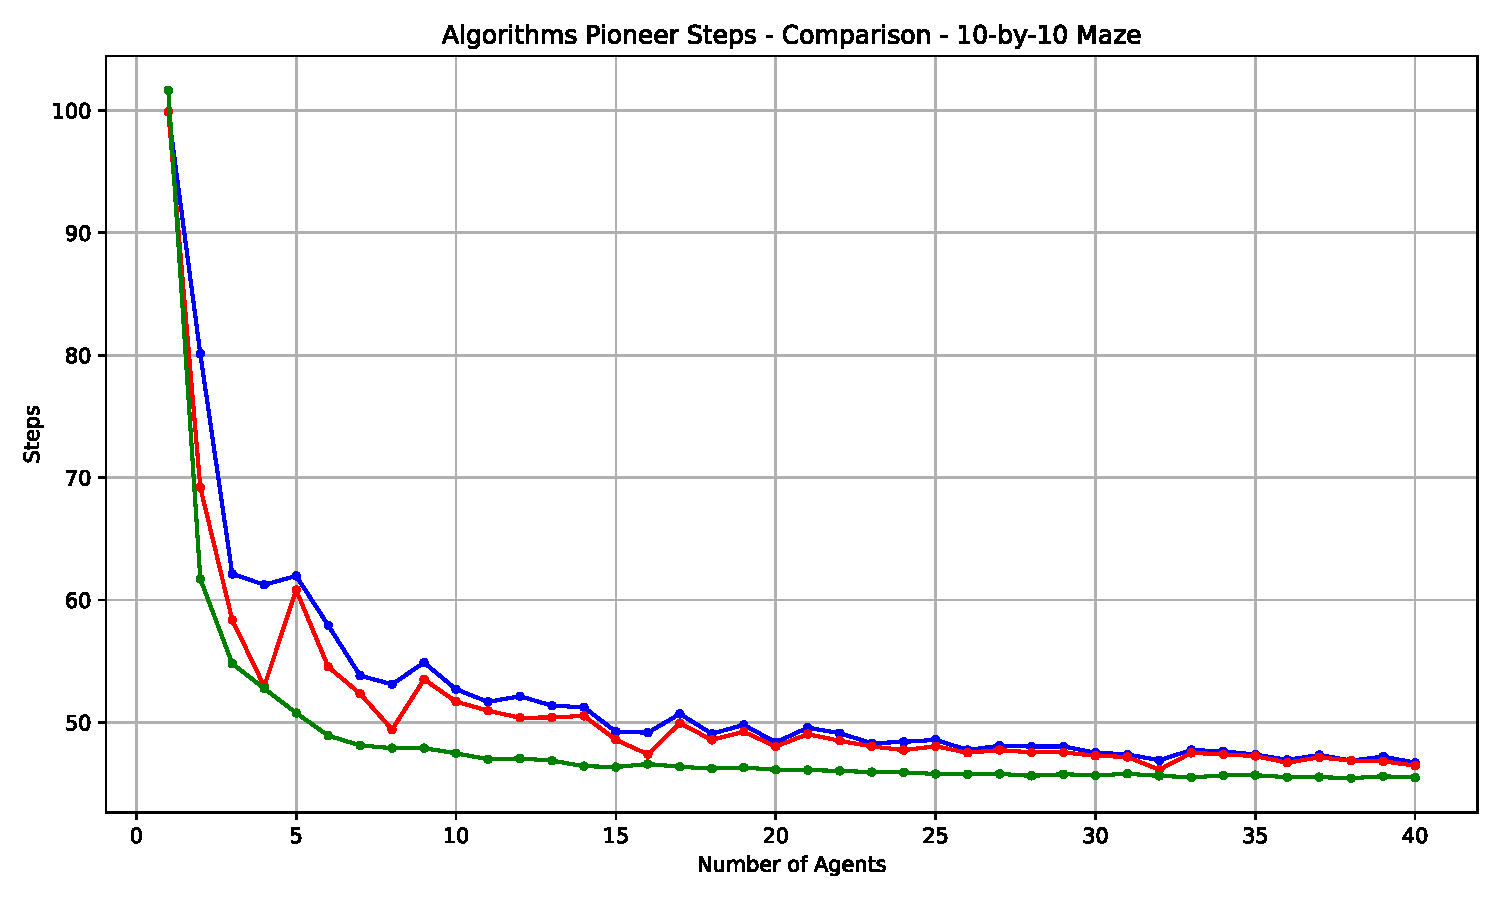
\includegraphics[width=\textwidth]{Cap3/no_comm_steps__10_by_10_maze.pdf}
        \caption{(a) 10x10 Maze}
        \label{fig_no_comm_steps_10x10_maze}
    \end{minipage}
    \hfill
    \begin{minipage}[b]{0.45\textwidth}
        \centering
        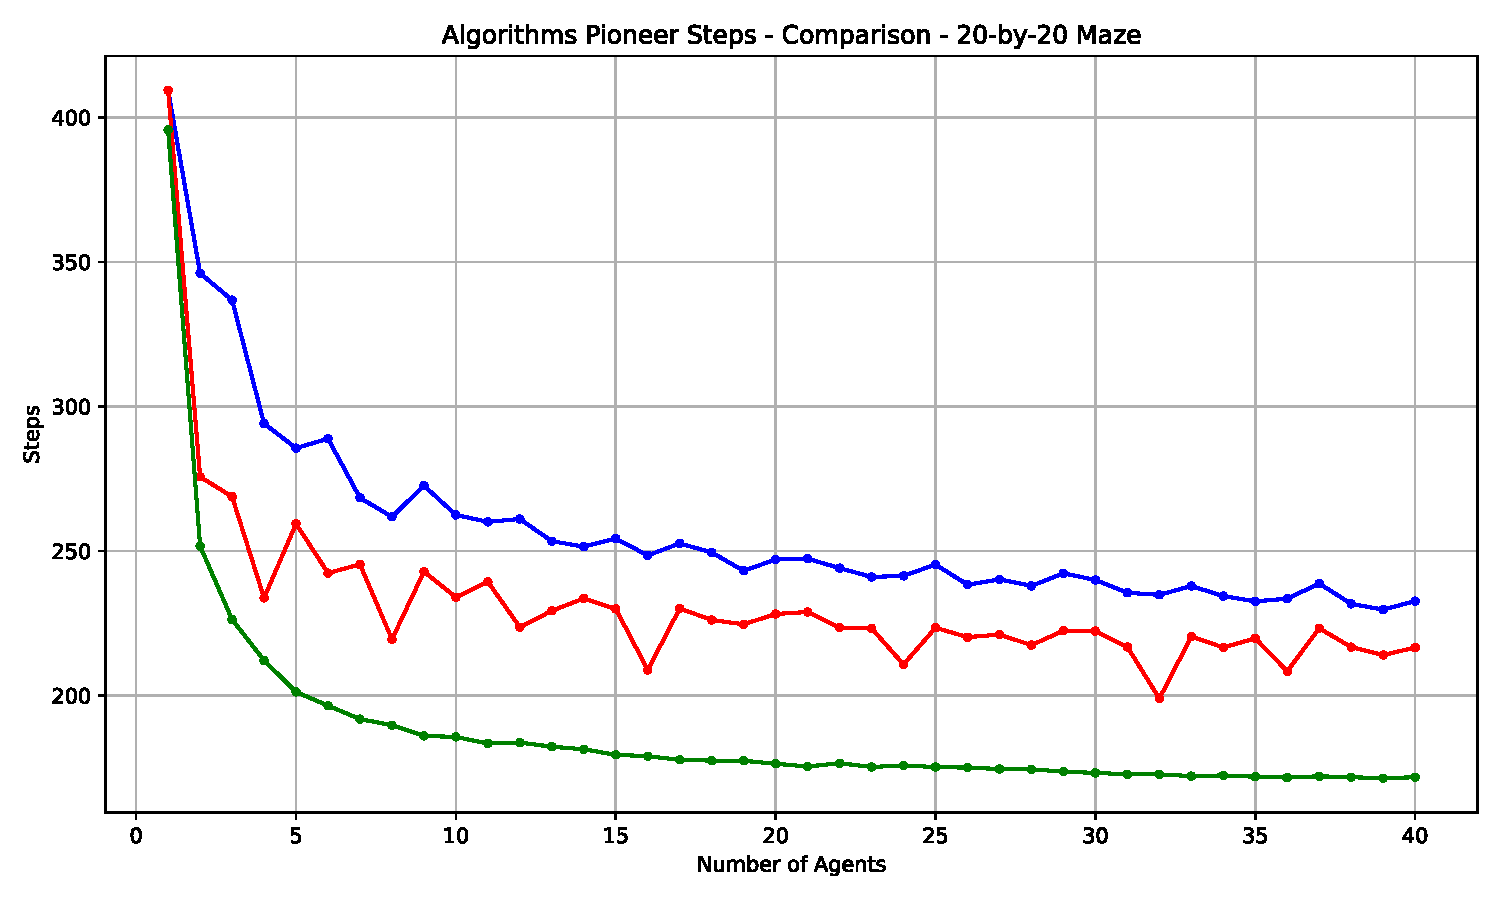
\includegraphics[width=\textwidth]{Cap3/no_comm_steps__20_by_20_maze.pdf}
        \caption{(b) 20x20 Maze}
        \label{fig_no_comm_steps_20x20_maze}
    \end{minipage}
    \vspace{1em}
    \begin{minipage}[b]{0.45\textwidth}
        \centering
        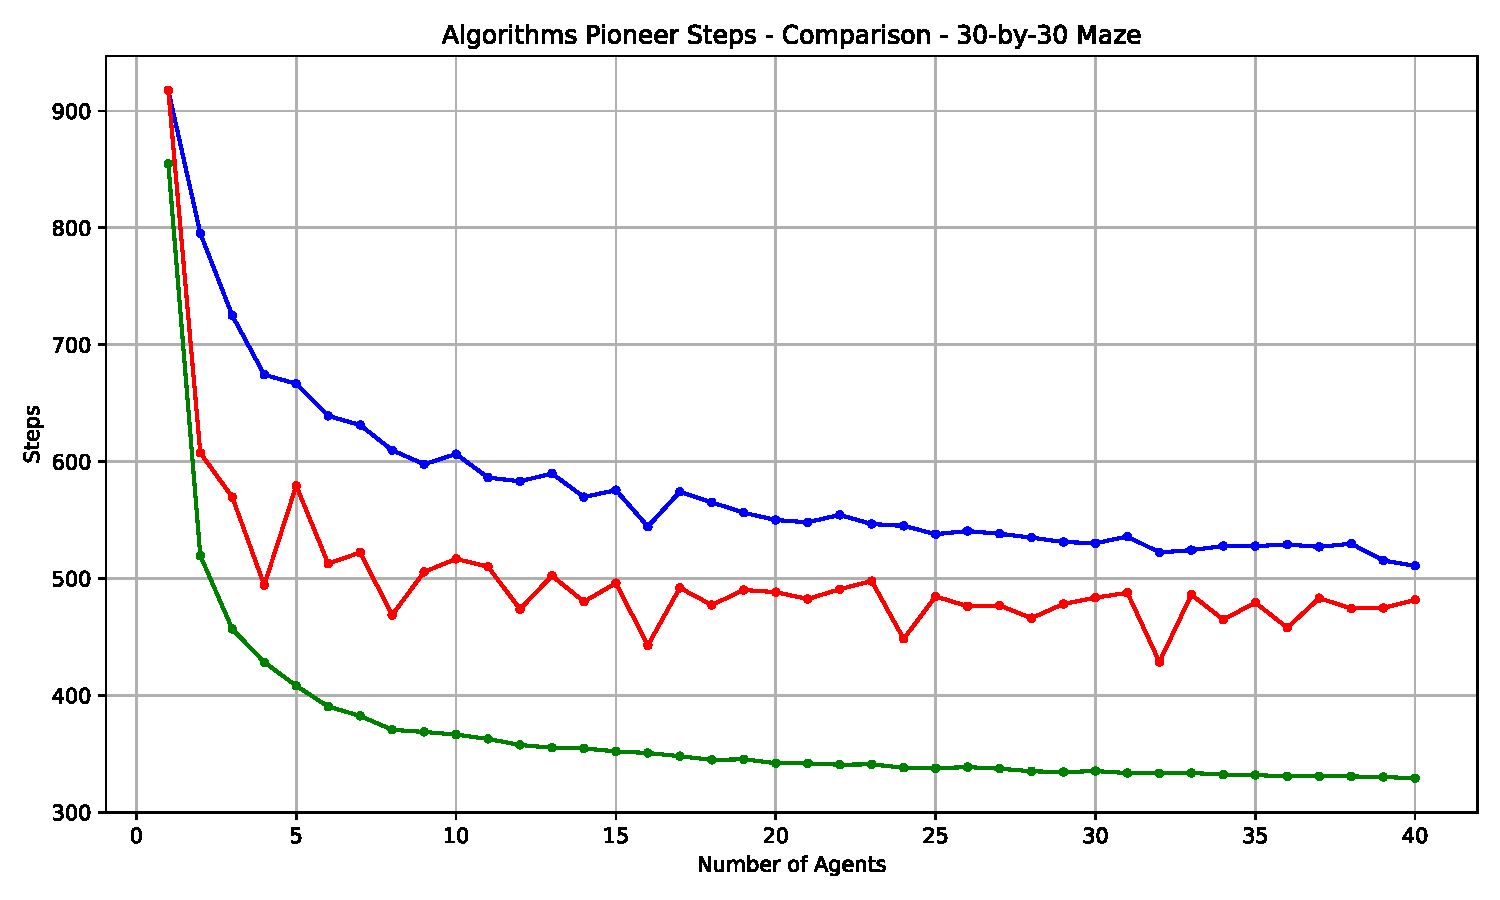
\includegraphics[width=\textwidth]{Cap3/no_comm_steps__30_by_30_maze.pdf}
        \caption{(c) 30x30 Maze}
        \label{fig_no_comm_steps_30x30_maze}
    \end{minipage}
    \hfill
    \begin{minipage}[b]{0.45\textwidth}
        \centering
        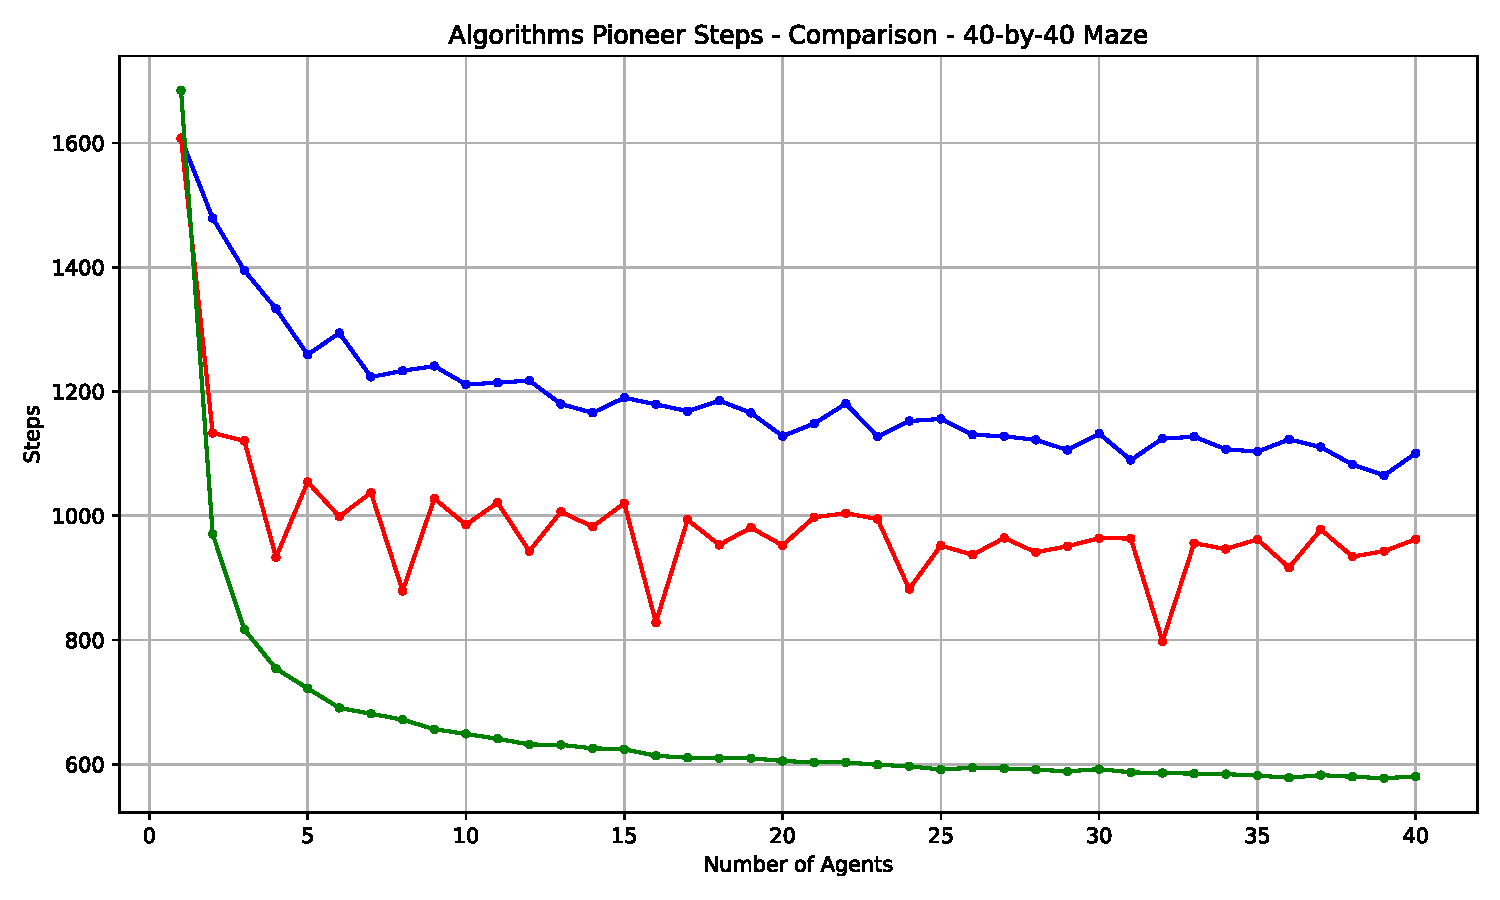
\includegraphics[width=\textwidth]{Cap3/no_comm_steps__40_by_40_maze.pdf}
        \caption{(d) 40x40 Maze}
        \label{fig_no_comm_steps_40x40_maze}
    \end{minipage}
    \caption{Comparison of the pioneer's average steps between our no-communication algorithms and the Tarry's algorithm across different sizes of perfect mazes. The subfigures illustrate how algorithm performance scales with maze size: (a) 10x10, (b) 20x20, (c) 30x30, and (d) 40x40.}
    \label{fig_no_comm_steps_all_sizes_maze}
\end{figure}

\begin{figure}[H]
    \centering
    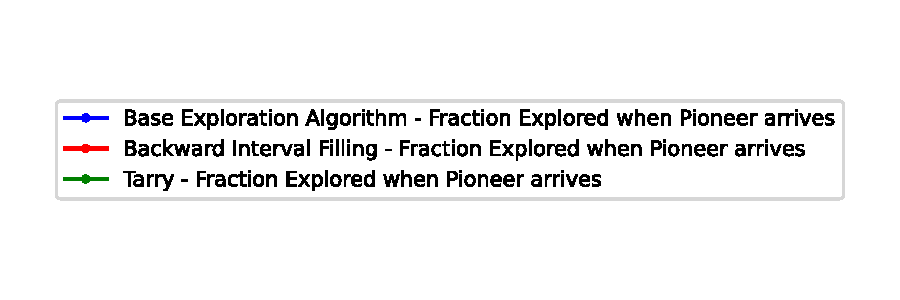
\includegraphics[width=0.8\textwidth]{Cap3/no_comm_fraction_legend.pdf}
    \vspace{1em}
    \begin{minipage}[b]{0.45\textwidth}
        \centering
        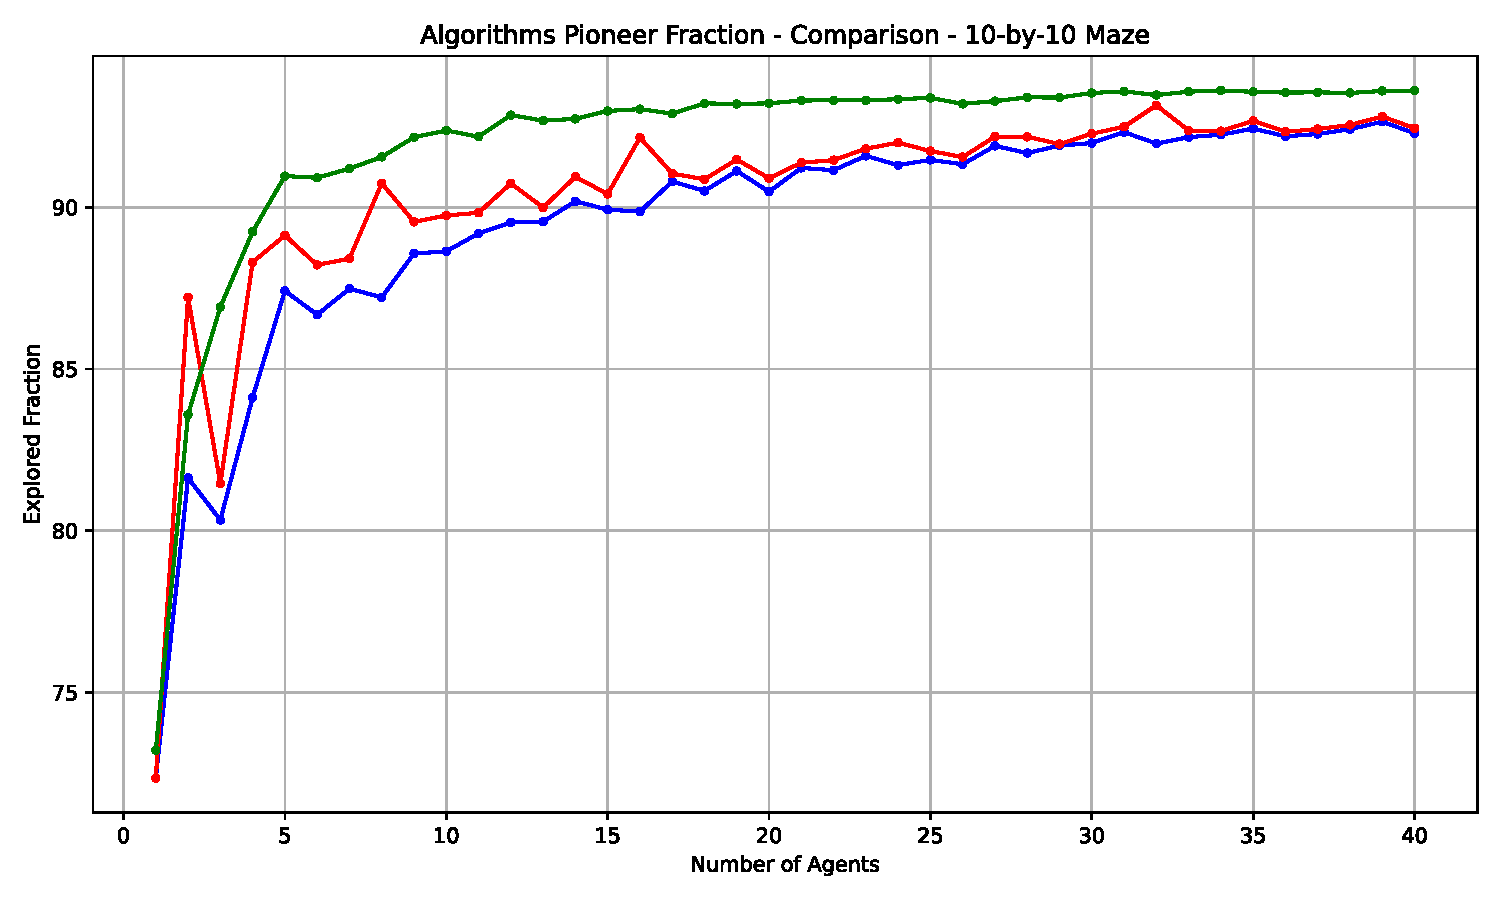
\includegraphics[width=\textwidth]{Cap3/no_comm_fraction__10_by_10_maze.pdf}
        \caption{(a) 10x10 Maze}
        \label{fig_no_comm_fraction_10x10_maze}
    \end{minipage}
    \hfill
    \begin{minipage}[b]{0.45\textwidth}
        \centering
        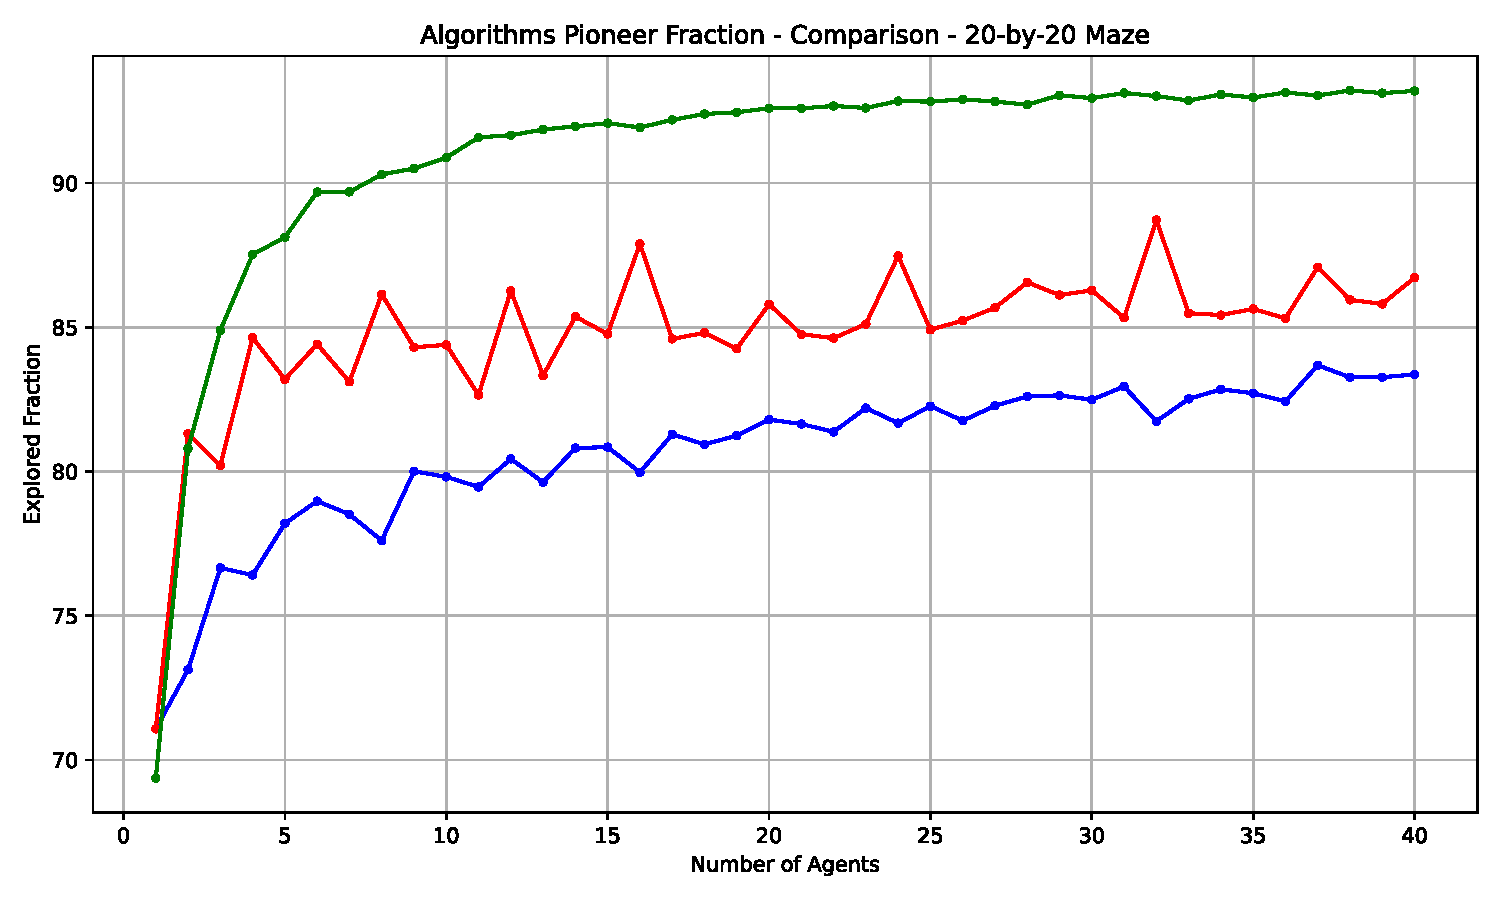
\includegraphics[width=\textwidth]{Cap3/no_comm_fraction__20_by_20_maze.pdf}
        \caption{(b) 20x20 Maze}
        \label{fig_no_comm_fraction_20x20_maze}
    \end{minipage}
    \vspace{1em}
    \begin{minipage}[b]{0.45\textwidth}
        \centering
        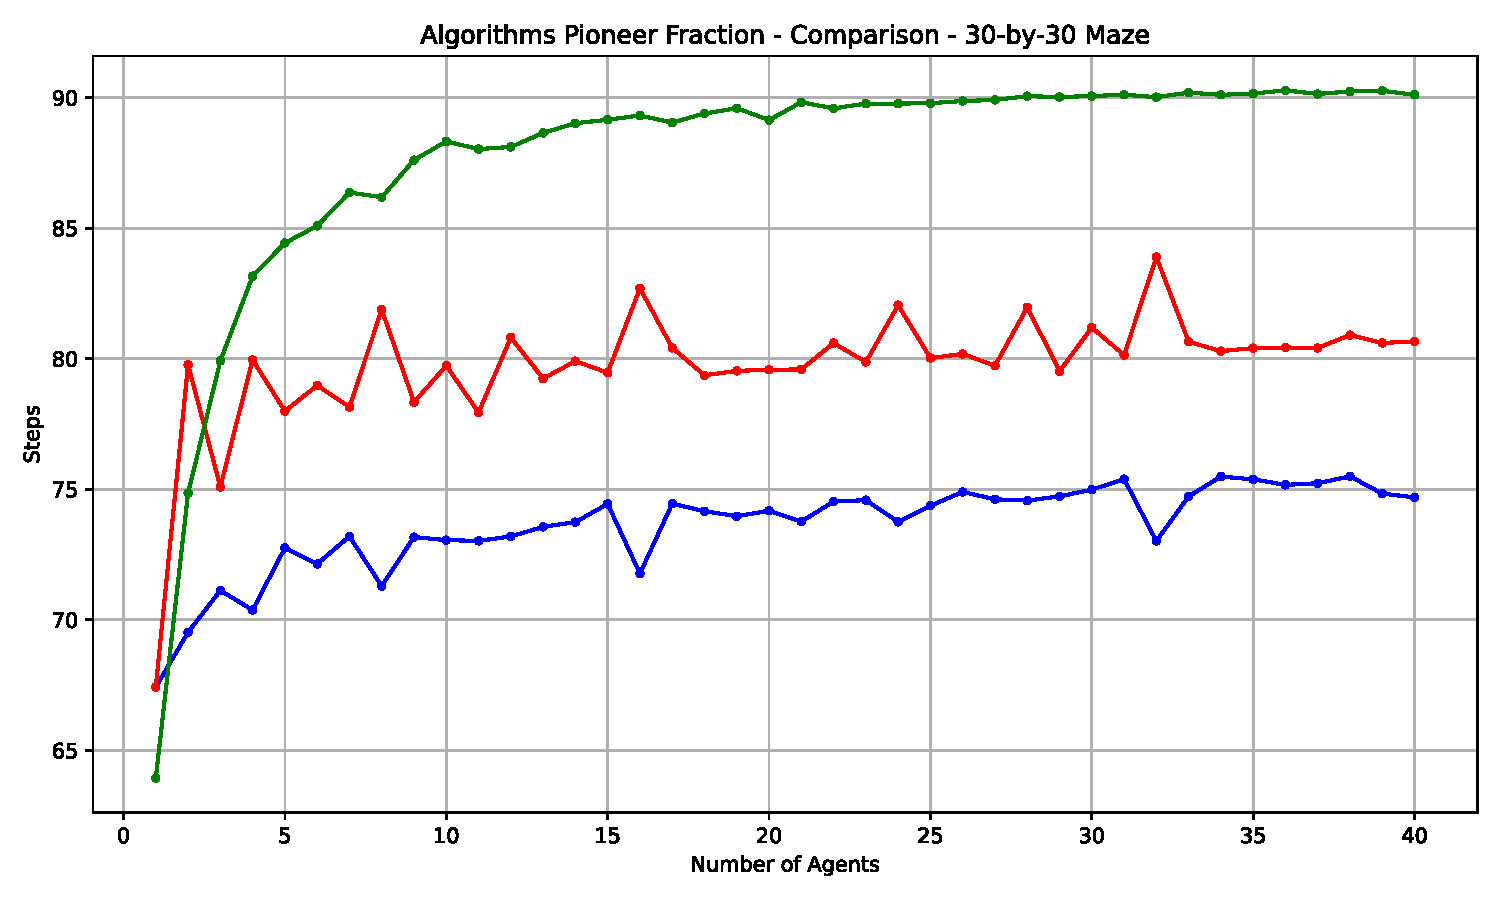
\includegraphics[width=\textwidth]{Cap3/no_comm_fraction__30_by_30_maze.pdf}
        \caption{(c) 30x30 Maze}
        \label{fig_no_comm_fraction_30x30_maze}
    \end{minipage}
    \hfill
    \begin{minipage}[b]{0.45\textwidth}
        \centering
        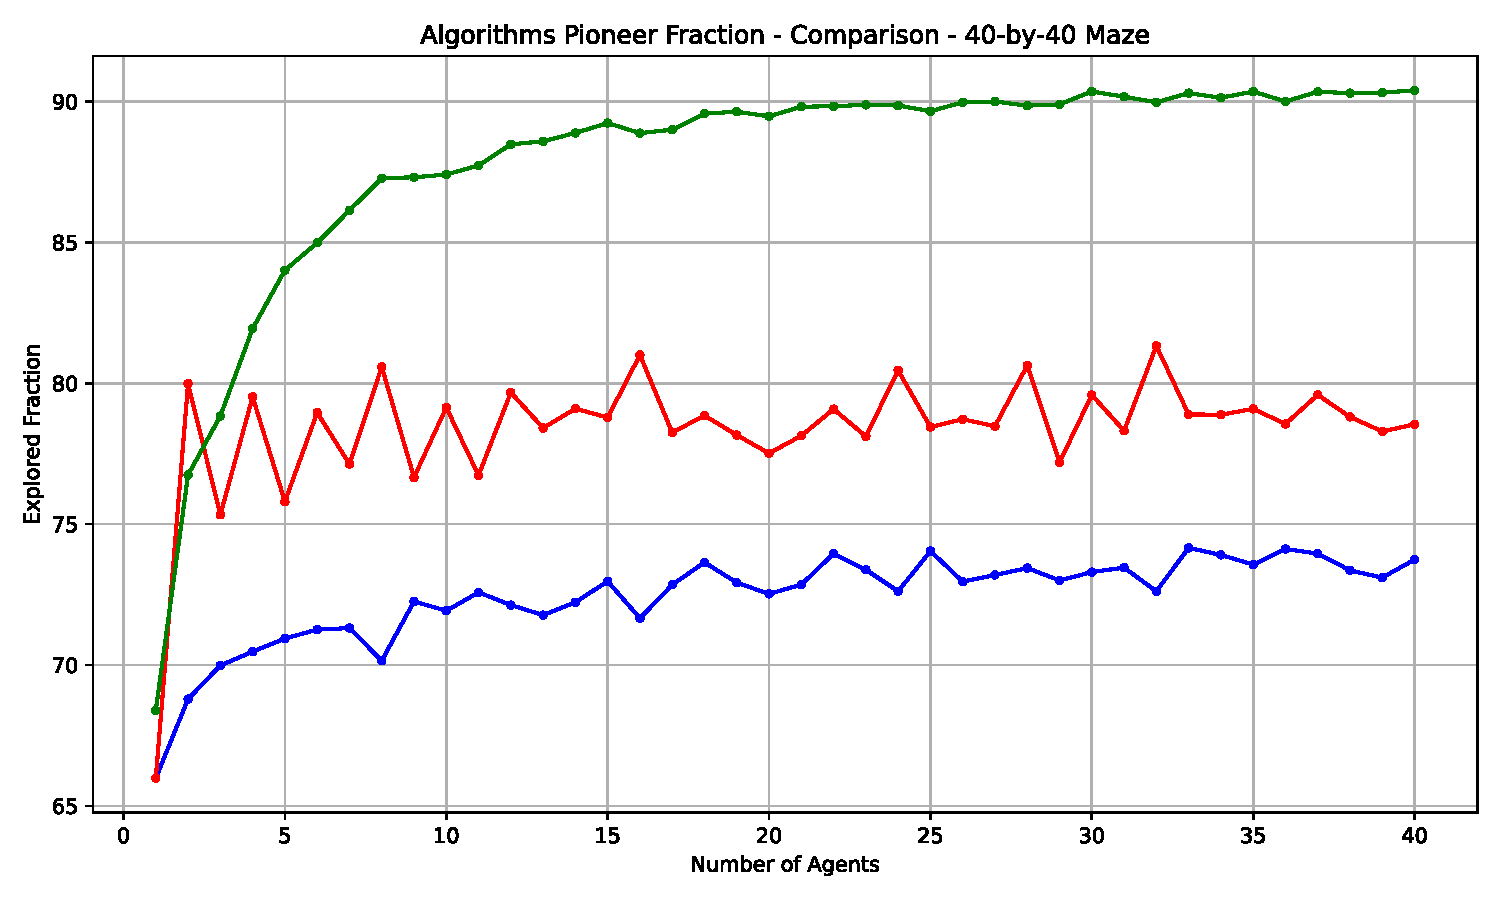
\includegraphics[width=\textwidth]{Cap3/no_comm_fraction__40_by_40_maze.pdf}
        \caption{(d) 40x40 Maze}
        \label{fig_no_comm_fraction_40x40_maze}
    \end{minipage}
    \caption{Comparison of the explored fraction achieved by our no-communication algorithms and Tarry's algorithm across different sizes of perfect mazes. The subfigures illustrate how coverage efficiency scales with maze size: (a) 10x10, (b) 20x20, (c) 30x30, and (d) 40x40.}
    \label{fig_no_comm_fraction_all_sizes_maze}
\end{figure}


The results show that adding more agents helps the pioneer find the goal cell faster, as the average number of steps taken decreases with more agents. This trend eventually levels off at a certain point when there are many agents. The explored fraction behaves similarly, with more agents spreading out quickly and covering more of the maze, though it also stabilizes over time. This outcome is expected, as more agents lead to quicker exploration and better coverage.

In addition to the expected results, the Backward Interval Filling algorithm shows a strange pattern when the number of agents is a power of two, starting from the 20x20 maze size. This matches earlier findings in \cite{Arthur2023}, but it hasn't been fully explored in previous studies. While we recognize the theory suggested by \citen{Arthur2023}, we did not investigate this behavior in detail in our research.

Building on these findings, we compared the performance of our no-communication algorithms with Tarry's algorithm. As expected, both Tarry's algorithm and the Backward Interval Filling variant perform better than the basic version of our algorithm. However, the level of improvement depends on the maze size. In larger mazes, Tarry's algorithm shows a bigger advantage. This is because, in smaller mazes, it's possible to quickly find the optimal solution by simply adding more agents. But in larger mazes, communication is crucial for avoiding repeated steps, which significantly enhances Tarry's performance.

\subsection{Random Tree Results} 
\label{subsection_no_comm_random_tree_results}

The results for the random trees of sizes 100, 500, and 1500 nodes are presented in Figure \ref{fig_no_comm_steps_all_sizes_tree}. These sizes were chosen because they effectively represent the trends observed across all tree dimensions without the need to include every possible size. Figure \ref{fig_no_comm_steps_all_sizes_tree} shows the steps taken by the pioneer, while the explored fraction is not displayed due to its high variability in trees, which could lead to misleading conclusions.

\begin{figure}[H]
    \centering
    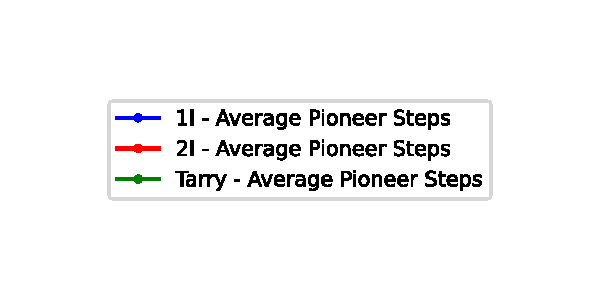
\includegraphics[width=0.8\textwidth]{Cap3/no_comm_steps_legend.pdf}
    \vspace{1em}
    \begin{minipage}[b]{0.45\textwidth}
        \centering
        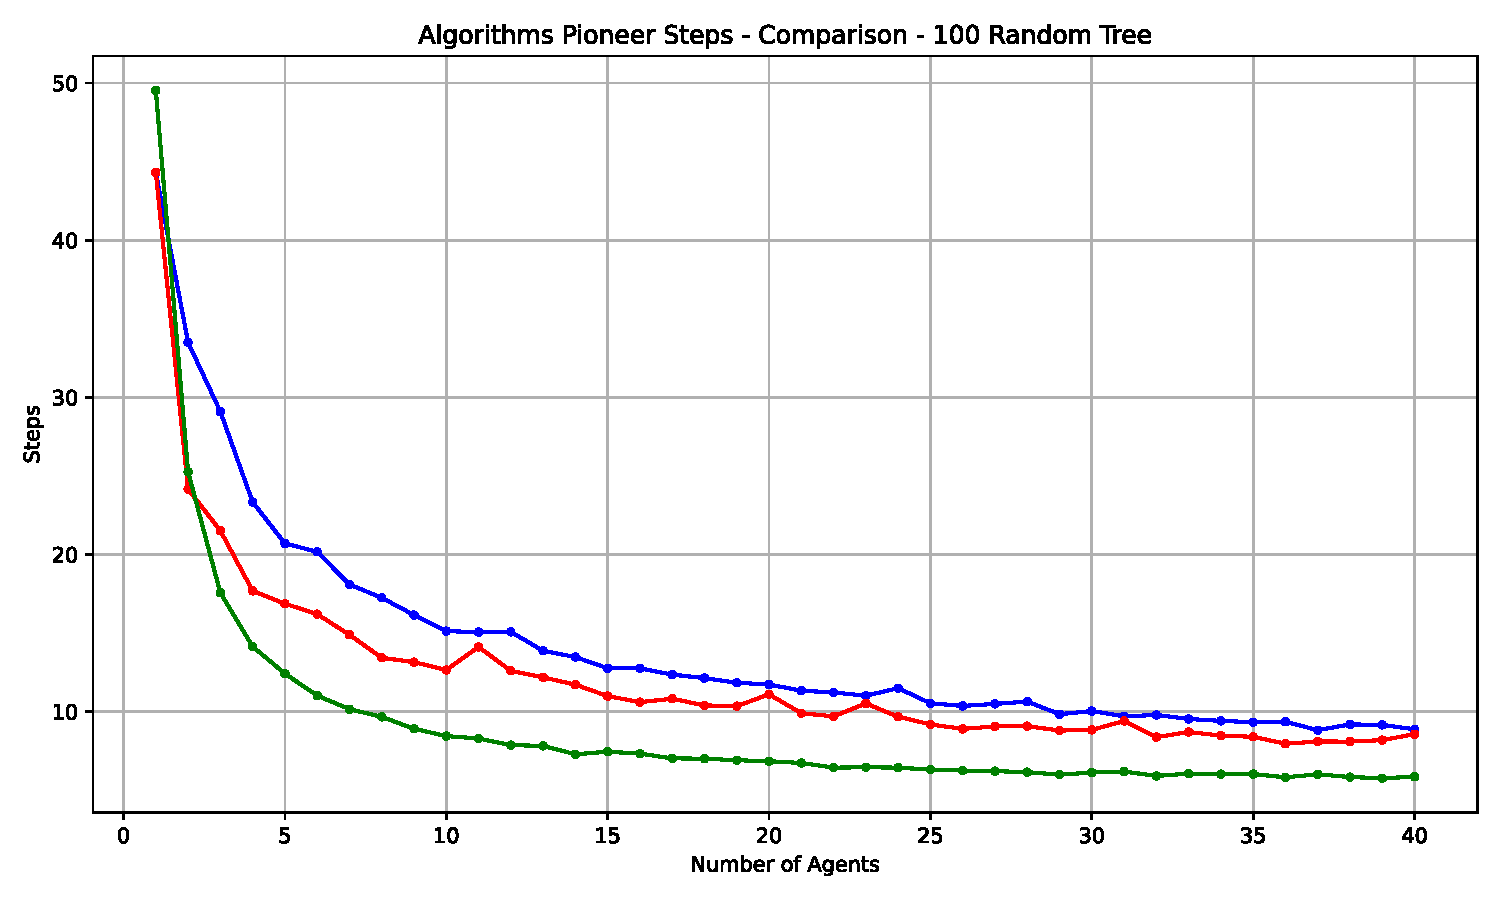
\includegraphics[width=\textwidth]{Cap3/no_comm_steps__100_tree.pdf}
        \caption{(a) 100-node Tree}
        \label{fig_no_comm_steps_100_tree}
    \end{minipage}
    \hfill
    \begin{minipage}[b]{0.45\textwidth}
        \centering
        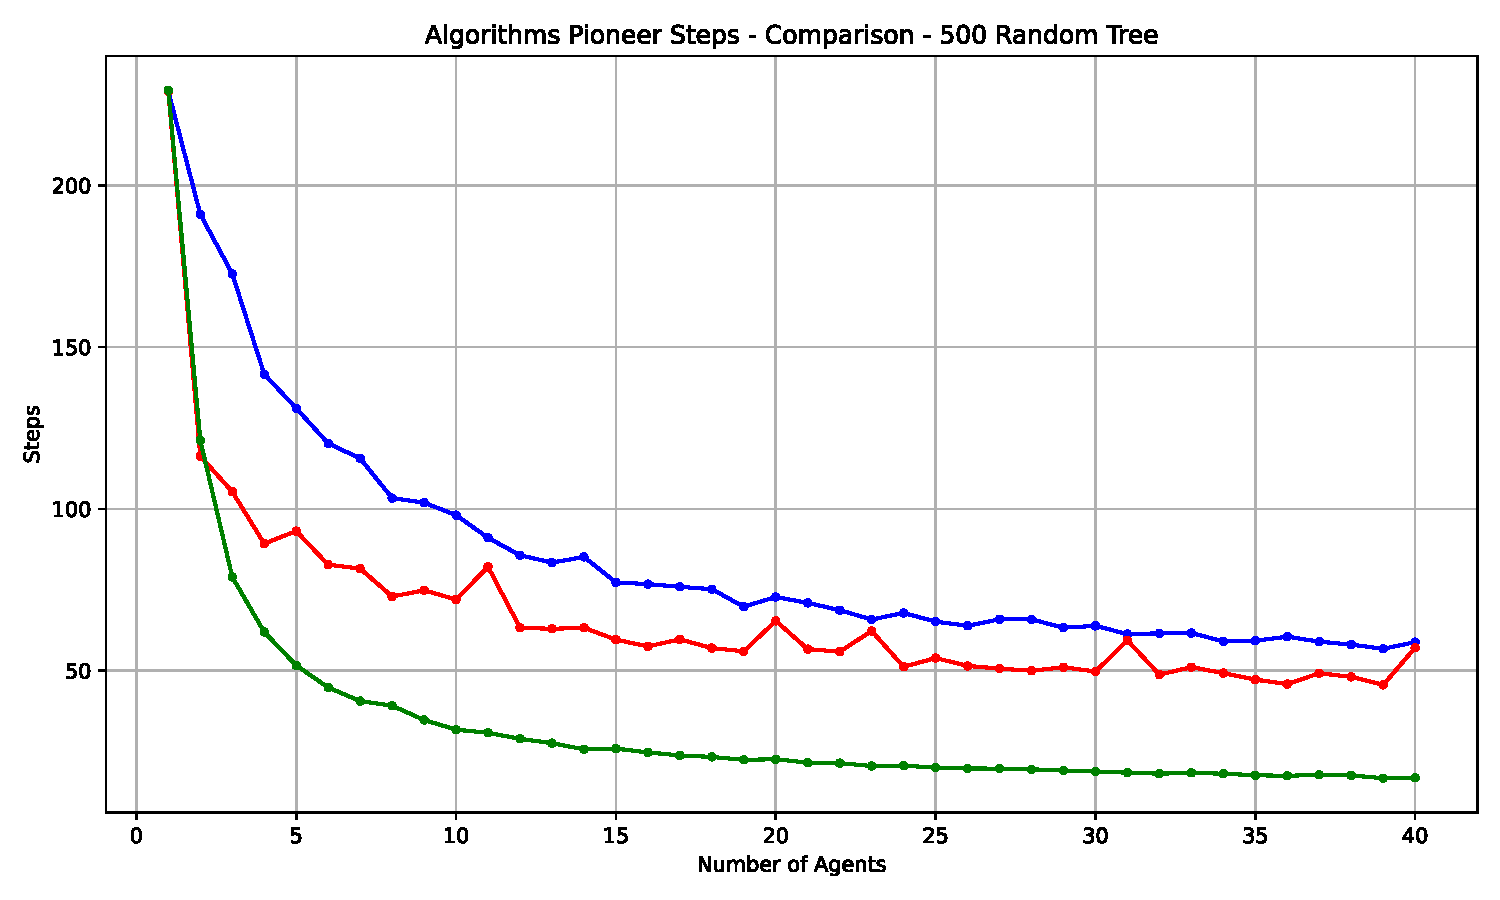
\includegraphics[width=\textwidth]{Cap3/no_comm_steps__500_tree.pdf}
        \caption{(b) 500-node Tree}
        \label{fig_no_comm_steps_500_tree}
    \end{minipage}
    \vspace{1em}
    \begin{minipage}[b]{0.45\textwidth}
        \centering
        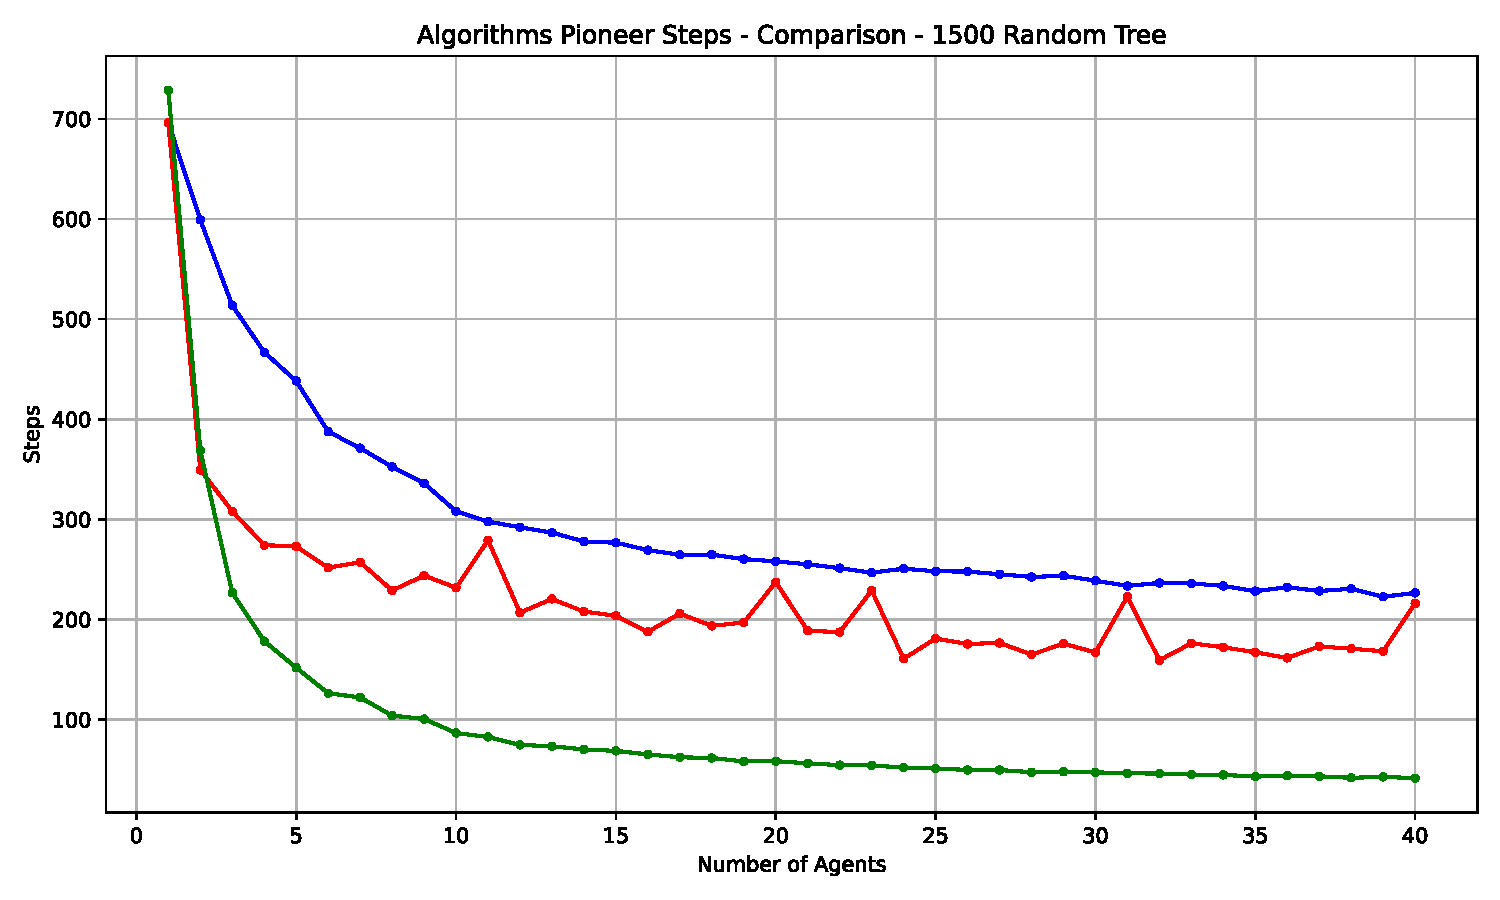
\includegraphics[width=\textwidth]{Cap3/no_comm_steps__1500_tree.pdf}
        \caption{(c) 1500-node Tree}
        \label{fig_no_comm_steps_1500_tree}
    \end{minipage}
    \caption{Comparison of the average steps taken by the pioneer across different no-communication algorithms and Tarry's algorithm for various sizes of random trees. The subfigures illustrate how algorithm performance varies with tree size: (a) 100 nodes, (b) 500 nodes, and (c) 1500 nodes.}
    \label{fig_no_comm_steps_all_sizes_tree}
\end{figure}

The results for the random trees confirm that the conclusions from Section \ref{subsection_no_comm_maze_results} still apply. Performance improves with more agents, Tarry's algorithm remains the most efficient, and its advantages increase with size.

Even though the trends hold, it's important to note that Tarry outperforms the Back Filling Interval Variation by approximately 39.6\% and our proposed algorithm by 47.3\% in the 40x40 maze. In contrast, in the 1500-node trees, Tarry shows a substantial improvement, being about 81.7\% better than our proposed algorithm and 80.8\% better than the Back Filling Interval Variation. This demonstrates the significant impact of dataset characteristics on the relative performance of our no-communication algorithms.


\section{Tarry's Variants Performance}
\label{section_result_tarry}

\subsection{Metrics for Analysis}
\label{subsection_tarry_metrics}

This section examines the results for Tarry's algorithm and its variants, specifically Tarry Tie-Breaker, Tarry Interval Priority, and Delayed Tarry.

In addition to the previously mentioned metrics in Section \ref{subsection_no_comm_metrics}, this section introduces a metric for the relative difference in performance compared to the base Tarry algorithm. This measure is particularly useful for interpreting results when the algorithms' performances are very close on some datasets, providing a clearer picture of the improvements or regressions.

\subsection{Perfect Maze Results} 
\label{subsection_tarry_maze_results}

\subsection{Random Tree Results} 
\label{subsection_tarry_random_tree_results}


    
    
    
    
    